%!TEX root = ../dissertation.tex
\chapter{Long coherent dynamics in optical lattices}

\section{Pure versus mixed states}
In order to understand what the purity of a state means and why it is important to be able to measure it, let's take a closer look at the difference between the quantum superposition and classically mixed states. While for both of them the measurements in most basis will lead to multiple different outcomes, for a pure quantum state there exists a basis in which a measurement will result in only one possible outcome. As an example, imagine that we have many copies of a spin $\frac{1}{2}$ particle, and we can measure each of them along any of the axes $x$, $y$, or $z$. If we had prepared half of the particles in a state $\left| \uparrow \right>$ and the other half in a state $\left| \downarrow \right>$ along the $z$ direction, the measurement in any of the bases will result in the $50/50$ split between the outcomes. Hence we will conclude that the state was mixed. Now, if the particles were initially prepared in the superposition state $(\left| \uparrow  \right>+ \left| \downarrow \right>)/\sqrt{2}$, the measurement along $y$ or $z$ would yield the same result. However, if we measure this state in the $x$ direction, we find that it produces only one of two possible outcomes. 

In terms of formal mathematical notations, it is useful to introduce a concept of a density matrix. Given a state $\left|\psi \right>$, the density matrix is defined as an outer product of the state with itself and can be formally written as $\rho_{\mathrm{pure}} = \left|\psi \right> \left< \psi \right|$. It is now easy to generalize this concept to include mixed states; they are just a incoherent sum of different pure states that occur  with certain probabilities and can formally be written as $\rho_{\mathrm{mixed}} = \sum_{i} c_{i}\left|\psi_{i} \right> \left< \psi_{i} \right|$, where $c_{i}$ is the probability of state $\left|\psi_{i} \right>$ so that $\sum_{i}c_{i}=1$. This gives us a very intuitive way of quantifying the purity of a given state by looking at the trace of the square of the density matrix. In the case of a pure state 
\begin{equation}
Tr(\rho_{\mathrm{pure}}^2) = Tr(\left|\psi \right> \left< \psi \right| \left|\psi \right> \left< \psi \right|) = Tr(\left|\psi \right> \left< \psi \right|) = Tr(\rho_{\mathrm{pure}})=1.
\end{equation}
On the other hand, if the state is mixed
\begin{equation}
Tr(\rho_{\mathrm{mixed}}^2) = Tr(\sum_{i} c_{i}\left|\psi_{i} \right> \left< \psi_{i} \right| \sum_{j} c_{j}\left|\psi_{j} \right> \left< \psi_{j} \right|) = Tr(\sum_{i} c^2_{i}\left|\psi_{i} \right> \left< \psi_{i} \right|) = \sum_{i} c^2_{i},
\end{equation}
and since there should be at least two non zero terms in this sum $Tr(\rho_{\mathrm{mixed}}^2) <1$. This means that by measuring the trace of the density matrix squared, we can quantify the purity of the state. 

Now let's consider what happens to the purity of a state, described by a density matrix $\rho$, during coherent time evolution. The time evolved density matrix can be written as $\rho(t) = U\rho(0) U^{\dagger}$, where $U$ is the unitary evolution operator, and hence 
\begin{equation}
Tr(\rho^2(t)) = Tr(U\rho(0) U^{\dagger} U\rho(0) U^{\dagger}) = Tr(U\rho(0) \rho(0) U^{\dagger}) = Tr(U^{\dagger} U\rho(0) \rho(0))  = Tr(\rho(0)^2). 
\end{equation}
This means that unitary evolution preserves the purity of the initial state. Since any coupling to the environment will result in a loss of purity, this also gives us a way to quantify how coherence of the system's dynamics is.

\section{Hong-Ou-Mandel effect}
In the next few sections, we will outline the procedure, that allows us to experimentally measure the purity of a quantum state. A more in-depth explanation can be found here \cite{PreissThesis}. In order to understand how this method works, it is instructive to consider the physics underlying the Hong-Ou-Mandel effect \cite{Hong1987}. The set up is the following: Consider two photons that are incident onto two different input ports of a perfect $50/50$ beamsplitter. Furthermore, let's suppose that they are identical to one another in every aspect, except for some parameter $\lambda$, which can be anything from photon frequency to the exact arrival time onto the beamsplitter (for simplicity let's assume that they have different wavelengths $\lambda_1$ and $\lambda_2$).

Mathematically, the beamsplitter transformation can be written in terms of creation and annihilation operators of the input modes i1, i2 and the output modes o1, o2 as
\begin{equation}
\begin{aligned}
& a_{i1}^{\dagger} \rightarrow (a_{o1}^{\dagger} + ia_{o2}^{\dagger} )/\sqrt{2} \\
& a_{i2}^{\dagger} \rightarrow (ia_{o1}^{\dagger} + a_{o2}^{\dagger} )/\sqrt{2}.
\end{aligned}
\end{equation}
When two photons are incident onto two different ports of the beamsplitter, the resulting state can be found as following:
\begin{equation}
\begin{split}
& a_{i1}^{\dagger}(\lambda_1) a^{\dagger}_{i2}(\lambda_2) \ket{0} \rightarrow  \frac{1}{2} (a_{o1}^{\dagger}(\lambda_1) +ia_{o2}^{\dagger}(\lambda_1) ) (ia_{o1}^{\dagger}(\lambda_2) +a_{o2}^{\dagger}(\lambda_2) )\ket{0} = \\
&=\frac{1}{2} (i a_{o1}^+(\lambda_1) a_{o1}^{\dagger}(\lambda_2) + ia_{o2}^{\dagger}(\lambda_1)a_{o2}^{\dagger}(\lambda_1) +a_{o1}^{\dagger}(\lambda_1) a_{o2}^{\dagger}(\lambda_2) - a_{o2}^{\dagger}(\lambda_1) a_{o1}^{\dagger}(\lambda_2))\ket{0},
\end{split}
\label{eq:BS}
\end{equation}
where $\ket{0}$ corresponds to a vacuum state. We can see that, in general, the beamsplitter results in $3$ possible states: $\ket{2,0}$, $\ket{0,2}$ and $\ket{1,1}$, where $\ket{m,n}$ represents a state with $m$ photons in the output port one and $n$ photons in the output port two of the beamsplitter. However, if the photon frequencies are identical, there is no way to determine the correspondence between the photons on the output port with those at the input and they become fundamentally indistinguishable. This is where the quantum nature of these particles comes into play. In this case the two last terms in the second line of equation~\ref{eq:BS} cancel each other, and the state $\ket{1,1}$ does not occur. This effect can be summarized as following: if two identical photons are incident onto a perfect $50/50$ beamsplitter the probability of simultaneously detecting a photon at each of the output ports equals zero. However, if the photons can be distinguished in some way, the probability of simultaneous detection becomes non-zero.

\section{Hong-Ou-Mandel interference of massive particles}
This effect can be also realized with massive bosonic particles and has first been observed in optical tweezers \cite{Kaufman2014} and momentum states of helium BECs \cite{Lopes2015}. One can understand it in the following way: Consider a double-well with a coupling strength $J$. The corresponding Hamiltonian reads 
\begin{equation}
H_{DW} = -J(a^{\dagger}_L a_R + a^{\dagger}_R a_L),
\end{equation}
where $a^{\dagger}_{L(R)}$ is bosonic creation operator for the left (right) site of the double-well. In the Heisenberg picture, this operators evolve under Hamiltonian dynamics, such that after an evolution time $t= \frac{2 \pi}{8J}$ the creation operators for the corresponding wells become
\begin{equation}
\begin{aligned}
& a_{L}^{\dagger} \rightarrow (a_{L}^{\dagger} +ia_{R}^{\dagger} )/\sqrt{2} \\
& a_{R}^{\dagger} \rightarrow (ia_{L}^{\dagger} +a_{R}^{\dagger} )/\sqrt{2}.
\end{aligned}
\end{equation}
Notice that if we define the left (right) well before the time evolution as input i1 (i2) and the same wells after the evolution as o1 (o2), this transformation becomes exactly identical to the beamsplitter one in equation \ref{eq:BS}. Hence, if we start with a single particle in each well, after the time evolution corresponding to the beamsplitter duration the probability of finding one particle in each well should be equal to zero. 

\begin{figure*}[t]
	\centering
	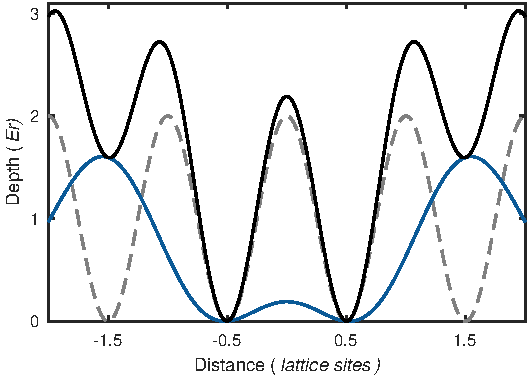
\includegraphics[scale=1]{figures/CBH_DW.pdf}
	\caption{{\bf Double-well potential for the beamsplitter operation}. The intensity profile of the DMD pattern (blue line) is combined with a shallow $2\mathrm{E_r}$ lattice (gray dashed line) to crate the double-well potential. Such configuration allows for isolated tunneling between two adjacent sites. Coupling to the neighboring site is strongly suppresed due to the potential offset of $1.7 \mathrm{E_{r}}. $}
	\label{fig:CBH_DW}
\end{figure*}

To observe this effect in our experiment, we prepare two atoms in the neighboring wells of our optical lattice. Using the DMD we isolate those wells by applying a repulsive potential, that detunes sites next to the double-well off-resonance for tunneling (see fig~\ref{fig:CBH_DW}). The exact shape of the DMD pattern is given by
\begin{equation}
V_{DW}(x) = (e^{-\frac{(x-1.5)^2}{\sigma_1^2}} - ae^{-\frac{(x)^2}{\sigma_2^2}} + e^{-\frac{(x+1.5)^2}{\sigma_1^2}})^2,
\end{equation}
where $x$ is measured in lattice sites. The values $\sigma_1 = 0.95$, $\sigma_2 = 0.9$, and a relative amplitude of the middle bump $a=0.52$ are chosen such that the offset between two minima of the resulting potential is linearly insensitive to a relative alignment of the DMD pattern with respect to the lattice, by having quadratic minimas at the location of the lattice sites. For our experiments, we superimpose a $2\mathrm{E_r}$ deep optical lattice with a $1.7\mathrm{E_r}$ deep DMD potential, resulting in the tunneling rate $J = 2 \pi \times 128 \mathrm{Hz}$.

\begin{figure*}[t]
	\centering
	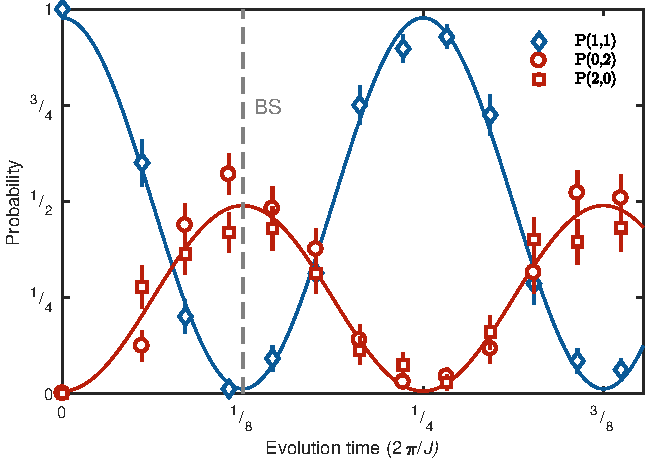
\includegraphics[scale=1]{figures/CBH_HOM.pdf}
	\caption{{\bf Tow particle osculations in the double-well potential}. The probability of the system to be in each of the $3$ available states as a function of time starting from initial state of one particle in each of the wells of the double-well. At the beamsplitter point (dashed line) the atoms undergo Hong-Ou-Mandel interference, where the probability of being in the $\ket{1,1}$ state goes to zero, while the other two states are populated equally. The solid lines show the fit to the data with residual probability $\mathrm{P}(1,1) = 0.02$ at the beamsplitter point.}
	\label{fig:CBH_HOM}
\end{figure*}

At the beginning of the experiment, atoms are held in a deep ($45 \textrm{Er}$) lattice that suppresses the tunneling. To enable the dynamics, we rapidly change the lattice depth to $2\textrm{Er}$ in $0.5\textrm{ms}$. The state of the double-well with two particles can be described in the basis of three configurational states: $\ket{1,1}$, $\ket{0,2}$, and $\ket{2,0}$, each corresponding to different arrangements of atoms between the two wells. In our experiment, we can measure the probability of the system occupying each of those states $P(1,1)$, $P(0,2)$, and $P(2,0)$ as a function of evolution time by using the previously described atom number resolved state readout procedure (see fig.~\ref{fig:CBH_HOM}). As we expect, after an evolution time of $t= \frac{2 \pi}{8J}$ the probabilities of the state $\ket{1,1}$ almost go to zero, whereas the probability of the states $\ket{0,2}$ and $\ket{2,0}$ are equal to each other. 

In our experiment, we observe a residual $\sim 2\%$ probability of the $\ket{1,1}$ state for a beamsplitter operation. This can be explained by the residual atom-atom interactions of $U=68\textrm{Hz}$ and an offset between the well of $\Delta = 20\textrm{Hz}$ in our system. We can determine these two parameters independently.

\section{Multi-particle case}
The Hong-Ou-Mandel effect can be also extended to the initial states with more than one particle. If we start with two identical $n\textrm{-particle}$ bosonic states, each at one of the input ports of the beamsplitter, the outcome would contain only states with an even number of particles in each of the output ports (this will be explained in the following sections). In particular, if we start with two particles in each of the input ports, the beamsplitter operation should result in
\begin{equation}
\ket{2,2}\rightarrow \sqrt{\frac{3}{8}}(\ket{4,0}+\ket{0,4})+\frac{1}{2} \ket{2,2}.
\end{equation}

The result of such an operation in our experiment is shown in the figure~\ref{fig:CBH_4particles}. In this case, our measured probabilities of the output states deviate from the theoretical prediction, which includes finite interaction strength and the offset between two wells. However, the discrepancy can be explained by the interaction assisted coupling to the higher bands in the axial direction of the lattice, which has relatively low trapping frequency.

\begin{figure*}[t]
	\centering
	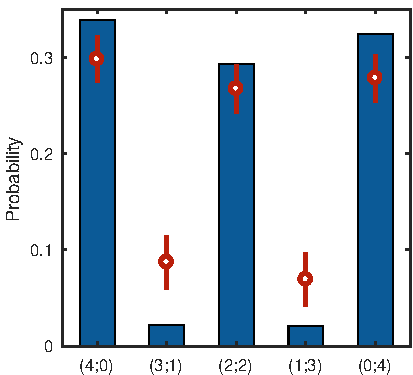
\includegraphics[scale=1]{figures/CBH_HOM_4particles.pdf}
	\caption{{\bf Four particle Hong-Ou-Mandel interference}. The probability of the system being in one of the five possible states at the beamsplitter point, starting with two particles in each well of the double-well. The bars show the prediction of exact digitalization for the experimental parameter regime of $\frac{U}{J}=0.53$ and relative offset of $\frac{\Delta}{J} = 0.15$. }
	\label{fig:CBH_4particles}
\end{figure*}

The interactions between particles within the same well modify the wave functions of individual particles, by making them wider compared to the non-interacting case. This, in turn, projects the single particle wave function onto the higher vibrational states of the harmonic trap in the axial direction, which makes the particles distinguishable between one another. To estimate this effect we assume that the exited band population of a single particle is proportional to $\epsilon \approx \left(\frac{U(n-1)}{2 \omega_z}\right)^2$, where $n$ is the number of particles on one site and $\omega_z$ is the trap frequency in the week direction. In the case of $4$ particles on the same site $\epsilon\sim0.017$, which should result in $\sim 6.5\%$ probability of odd outcomes. Combined with $\sim 4.3\%$ of odd outcomes due to the finite interaction strength within the single band model leads to the total of $\sim 10.8\%$ probability of odd outcomes, which is within the errorbar of our measurement (see fig.~\ref{fig:CBH_4particles}).

\section{Many-body interference as a measure of indistinguishability}
In order to generalize the Hong-Ou-Mandel idea to arbitrary, bosonic many-particle states, let's consider a system consisting of two states $\ket{\psi}_1$ and $\ket{\varphi}_2$. The full wave function $\ket{\psi}_1 \otimes \ket{\varphi}_2$ can be written in terms of creation operators $a_{1(2)}^{\dagger}$ acting on the subspaces $1$ $(2)$ as
\begin{equation}
\ket{\psi}_1 \otimes \ket{\varphi}_2 = \frac{1}{(\sqrt{2})^{p+q}}(a^{\dagger}_1 + a^{\dagger}_2)^p(a^{\dagger}_1 - a^{\dagger}_2)^q\ket{0},
\end{equation}
where $\ket{0}$ is a vacuum state.

If two states $\ket{\psi}_1$ and $\ket{\psi}_2$ are identical the full state $\ket{\psi}_1 \otimes \ket{\psi}_2$ should be symmetric under the exchange of particles between $1$ and $2$ ($a_{1}^{\dagger} \leftrightarrow a_2^{\dagger}$), due to the symmetry of the bosonic wave function. Hence, the antisymmetric part of the wave function should be raised to an even power
\begin{equation}
\ket{\psi}_1 \otimes \ket{\psi}_2 = \frac{1}{(\sqrt{2})^{p+q}}(a^{\dagger}_1 + a^{\dagger}_2)^p(a^{\dagger}_1 - a^{\dagger}_2)^{2m}\ket{0}.
\end{equation}

Notice, that by applying a unitary transformation given by
\begin{equation}
\begin{aligned}
& (a_{1}^{\dagger} + a_{2}^{\dagger} )/\sqrt{2} \xrightarrow[]{\text{DFT}} a_{1}^{\dagger} \\
& (a_{1}^{\dagger} - a_{2}^{\dagger} )/\sqrt{2} \xrightarrow[]{\text{DFT}} a_{2}^{\dagger},
\end{aligned}
\label{eq:DFT}
\end{equation}
we will transform our state into $\ket{\psi}_1 \otimes \ket{\psi}_2 \xrightarrow[]{\text{DFT}} (a^{\dagger}_1)^p (a^{\dagger}_2)^{2m}\ket{0}$. This means that application of such transformation to two identical states results in the even number of particles in the corresponding subspace. Therefore, it can serve as a probe of indistinguishability between two quantum states. The transformation described by the equation~\ref{eq:DFT} corresponds a two point version of the discrete Fourier transform (DFT), and the results in the following sections can be generalized to higher order correlation functions by considering multi-point DFTs \cite{Daley2012}.

The DFT transformation is very similar to the beamsplitter operation given by equation~\ref{eq:BS}. In fact, the beamsplitter can be reduced to the DFT by applying local $\frac{\pi}{2}$ phase shifts on one of the input ports of the beamsplitter. However, if two states have no defined phase relations, such as fixed particle number states, both operations are equivalent to one another. That's why applying the beamsplitter to the photon number states allows us to tell if the states were identical or not. In our experiment, we always work with fixed particle number states, which allows us to use the beamsplitter transformation instead of the DFT as well. 

\section{Measuring the purity of a state}
To understand how the DFT allows us to measure the purity of a given state, let's introduce one more useful concept called the $SWAP$ operator. It is defined as following: Consider two states $\ket{\psi}_1$ and $\ket{\varphi}_2$, $SWAP$ acting on a tensor product of the two results in 
\begin{equation}
SWAP(\ket{\psi}_1 \otimes \ket{\varphi}_2) = \ket{\varphi}_1 \otimes \ket{\psi}_2.
\end{equation}
Since applying $SWAP$ twice returns the state to itself, the eigenvalues of the operator are $\pm 1$, and the corresponding eigenstates can be written as $(a^{\dagger}_1 \pm a^{\dagger}_2)/\sqrt{2}$ in terms of creation operators in each subspace. As we have shown above, DFT will map the antisymmetric eigenstate onto a creation operator in the corresponding subspace (see eq.~\ref{eq:DFT}). Thus, by measuring the particle number in that subspace after the DFT, we can determine the eigenvalue of the $SWAP$ operator (even numbers corresponding to $+1$ and odd to $-1$). This means, that if we would like to measure the expectation value of the $SWAP$ operator with respect to a product state of two density matrices $\rho^{(1)} \otimes \rho^{(2)}$, we can do it by measuring the atom number parity of the appropriate subspace after performing the DFT
\begin{equation}
Tr(SWAP(\rho^{(1)} \otimes \rho^{(2)})) \xrightarrow[]{\text{DFT}} \left< P_2 \right>,
\end{equation}
where $\left< P_2 \right>$ is average parity in the second subspace.

The final step is to connect the expectation value of the $SWAP$ to the quantum state overlap \cite{Ekert2002}, which for two states described by the density matrices $\rho^{(1)}$ and $\rho^{(2)}$ is given by $Tr(\rho^{(1)} \rho^{(2)})$. To see this, consider the following:
\begin{equation}
\begin{aligned}
Tr(SWAP(\rho^{(1)} \otimes \rho^{(2)})) =& Tr(SWAP(\rho^{(1)}_{ij} \rho^{(2)}_{kl} \ket{i}\bra{j} \otimes \ket{k}\bra{l})) =Tr(\rho^{(1)}_{ij} \rho^{(2)}_{kl} \ket{k}\bra{j} \otimes \ket{i}\bra{l}) = \\
&=\sum_{ijkl}\rho^{(1)}_{ij} \rho^{(2)}_{kl} \delta_{kj} \delta_{il} = \sum_{ik}\rho^{(1)}_{ik} \rho^{(2)}_{ki} = Tr(\rho^{(1)} \rho^{(2)}).
\end{aligned}
\end{equation}
In particular, if $\rho^{(1)}=\rho^{(2)}=\rho$, then the state overlapped with itself leads to the purity \cite{Alves2004, Daley2012} $Tr(\rho^{(1)} \rho^{(2)}) = Tr(\rho^2)$.

Let's summarize the conclusions above: In order to measure the purity of a state described by the density matrix $\rho$, we need to prepare two identical copies of the same state, perform DFT on them, and finally measure average particle parity in one of the subspaces
\begin{equation}
Tr(\rho^2) = Tr(\rho\rho) = Tr(SWAP(\rho \otimes \rho)) \xrightarrow[]{\text{DFT}} \left< P_2 \right>.
\end{equation}
Moreover, for the states without a defined phase relation (such as fixed particle number states) any unitary transform that splits the particles equally between two subspaces can play the role of DFT (for instance a beamsplitter operation).

\section{Multi-mode systems}
So far we have only discussed the situation where the state of interest occupies a single bosonic mode (i.e. can be written as a polynomial function of a single creation operator $a^{\dagger}$ acting on the vacuum). However, in general, the states can occupy multiple modes at the same time. For example, consider a bosonic particle on a lattice that is delocalized over all sites of the lattice. Its state, up to a normalization, can be written as $\ket{\psi} = \sum_i a_i^{\dagger} \ket{0}$, where $a_i^{\dagger}$ is a creation operator on the i-th site of the lattice. This means that in the scheme described above we have to perform the DFT on each mode available to the system (i.e. in this case on each every lattice site). For our experimental implementation, it means that we have to perform a beamsplitter operation between the corresponding sites of each of the copies. In order to compute the overall parity of a given realization, we can simply take the product of the parities of individual modes $\left<P_{full}\right> = \left< \prod_i P_i \right>$, where $i$ runs through all modes of the system (see fig.~\ref{fig:CBH_multy_mode}).

\begin{figure*}[t]
	\centering
	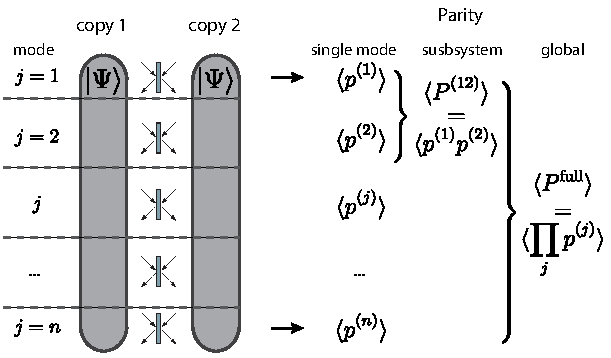
\includegraphics[scale=1]{figures/CBH_multimode.pdf}
	\caption{{\bf Parity of a multi-mode system}. In order to compute the total parity of the multi-mode system we need to multiply the parities of individual modes and then average the product over the realizations. By defining a subsystem as certain subset of modes we can compute the parity associated with that particular subsystem by taking the product over the corresponding modes.}
	\label{fig:CBH_multy_mode}
\end{figure*}

The multi-mode structure of a state additionally enables us to measure the purity of the subsystem, which can be defined as a certain subset of modes within the state. By averaging the parity only among those $\left<P_{sub}\right> = \left< \prod_{i \in sub} P_i \right>$ we will obtain the purity of the given subsystem.  Importantly, we can obtain the purity of any subsystem through data processing, by simply blinding ourselves to the outcomes of the beamsplitters that do not belong to the subsystem of interest. This will be very important later on when we will discuss the measurement of entanglement within the system.

\section{Decoherence between copies}
Although being a powerful tool to measure the purity of the system, many-body interference has one crucial limitation. Since the method measures the state overlap between two copies, it results in the purity only if two states are exactly identical. This task becomes even more challenging if we are interested in dynamical measurements because we have to ensure that both the initial states of the two copies as well as Hamiltonians under which each copy is evolving are identical to each other.

\begin{figure}[t]
	\centering
	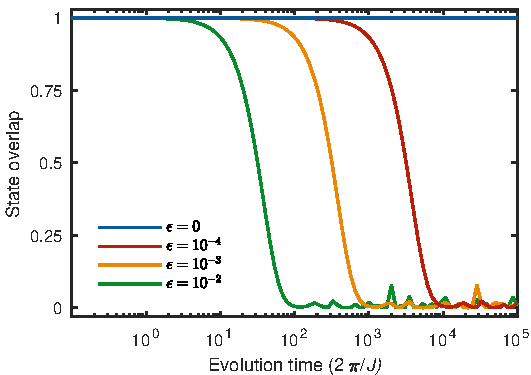
\includegraphics[scale=1]{figures/CBH_overlap.pdf}
	\caption{{\bf Dephasing of two many-body states}. Quantum state overlap $Tr(\rho_1 \rho_2) $ between two states that evolve under slightly different Hamiltonians, for which the difference in tunneling strength is parametrized be the parameter $\epsilon = \frac{\Delta J}{J}$. The overlap remains near unity until the time given by $\tau = 10^{log(\epsilon)-1}$, when it decays to zero after $\sim 1$ decade of time evolution.}
	\label{fig:CBH_overlap}
\end{figure}

In order to understand these effects, we perform numerical studies in the parameter regime corresponding to our experiment. We consider the scenario where two system starts in the same initial state but evolve under slightly different Hamiltonians. For these simulations, we work with one-dimensional $8$ site-long Bose-Hubbard chain with $U/J\sim1$. The initial state is a charge-density wave at half filling. To make the Hamiltonians between two copies different the tunnelling strength in the second one is set to be $J_2 = J_1(1+\epsilon)$, where $\epsilon \ll 1$. The tunnelling strength also provides a natural time scale for the problem given by $\frac{2 \pi}{J}$.

As we expect, if $\epsilon = 0$ then two copies remain identical throughout the whole evolution time, resulting in the state overlap $Tr(\rho_1 \rho_2) = 1$ (see fig.~\ref{fig:CBH_overlap}). However, if $\epsilon > 0$ state overlap remains at $1$ up to some time scale, but then decays to zero over about one decade of time evolution. From the numerical data, we can identify that the deviation from unity overlap occurs at a timescale given by $\tau = 10^{log(\epsilon)-1}$. From this analysis, we can conclude that, as long as we look at the timescales shorter than $\tau$, many-body interference results in the purity of the state. However, it also imposes a challenge for the experiments, if we would like to do measurements on very long timescales.

% Intuitively this result can be understood as fallowing: Consider two Hamiltonians $H^{(1)}$ and $H^{(2)}$ such that their ordered eigenvalues are very close to each other 
%\begin{equation}
%|\lambda^{(1)}_i-\lambda^{(2)}_i|<\epsilon},
%\end{equation}
%where $\epsilon \ll 1$. Since the eigenvalues are similar  some initial state $\ket{\psy_0}$

\begin{figure}[t]
	\centering
	\includegraphics[scale=1.2]{figures/ETH_protocol.pdf}
	\caption{{\bf Experimental sequence.} Using cutting techniques, we deterministically prepare two copies of a six-site Bose-Hubbard system, where each lattice site is initialized with a single atom. We suddenly switch on the tunnelling in the x-direction and obtain a highly excited state in each six-site copy, populating a large fraction of the many-body eigenstates. After a variable evolution time, we freeze the dynamics along the chains and characterize the final quantum state overlap between two copies by performing the beamsplitter operation.}
	
	\label{fig:CBH_purity_protocol}
\end{figure} 

In order to characterize our system, we perform the following experiment (see fig.~\ref{fig:CBH_purity_protocol}): First, we prepare two copies of an unentangled product state, consisting of a chain of $6$ atoms in the $45\mathrm{E_r}$ deep lattice in both directions. Next, we confine our system to the desired size (for this experiment either $6$ or $12$ sites long), by detuning the sites outside the region, in a similar way as for the beamsplitter experiments. Then, we rapidly drop the lattice along the chains, allowing atoms to tunnel. After a variable evolution time, we suddenly freeze the dynamics by increasing the lattice depth. Till this point, the lattice between the copies stays high such that the two states evolve independently from each other. Finally, we perform the beamsplitter operation between two copies, by dropping the lattice between them and allowing for tunnelling corresponding to the beamsplitter time. At the end of the experiment, we perform atom-number-resolved readout of the whole system.

\begin{figure*}[t]
	\centering
	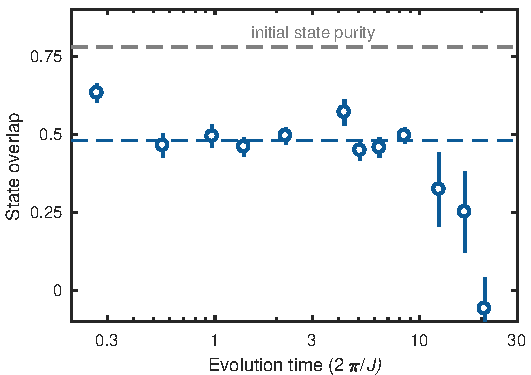
\includegraphics[scale=1]{figures/CBH_MBP_single_trace.pdf}
	\caption{{\bf Many-body coherence between two copies}. Quantum state overlap $Tr(\rho_1 \rho_2) $ between two six sites chains in our experiment shows a steady state between $0.5-10$ tunneling times. The reduction of purity is consistent with non-perfect beamsplitter operation, therefore, we conclude that two copies remain coherent up to $\sim10$ tunneling times. }
	\label{fig:CBH_MBP_vs_time}
\end{figure*}
\label{bs_imperfactions}
The initial state of the system is a product state of a single atom on every site of the chain in each copy. Hence, the application of a many-body beamsplitter is equivalent to the product of $6$ individual beamsplitters with one particle in each well of the double-well. In this case, each beamsplitter operation leads to a HOM interference, resulting in an average purity of $78.3(1)\%$ for the full state, limited by our beamsplitter imperfections (see fig.~\ref{fig:CBH_MBP_vs_time}). Once we switch on the tunnelling along the chains, the purity of the state decreases until it reaches a stationary value between $0.4$ and $ 9$ tunnelling times. Starting at $\sim 10$ tunnelling times the purity drops from this stationary value all the way to zero. We attribute this decay to the decoherence between two copies.

The initial decay of purity is attributed to the fact that the system is evolving to a state with high single-site atom-number occupation. As was discussed in the previous sections, our HOM contrast is decreased for states with higher on-site atom-number, leading to an increased likelihood of non-perfect interference. We can estimate this effect in the following way: In the stationary regime, the on-site number distribution can be approximated as having $35\%$, $40\%$ and $25\%$ probability of having zero, one and two particles respectively. The beamsplitter results in the purity of $1$, $0.96$ and $0.7$ for the respective values. Computing the result of the full beamsplitter operation on $6$ sites with the above distribution results in an overall purity of $0.53$, which is very close to the measured value.

\section{Increasing the coherence of the system}
In order to improve the coherence in the systems, we can do either of two things: make the Hamiltonians in both copies more identical to one another or decrease the characteristic \linebreak timescale of the experiment given by the tunnelling strength. The difference between two Hamiltonians comes from the imperfections in our optical lattice potential that occur due to the interference of the lattice beams with the stray light. Therefore, the amount of disorder in absolute units decreases with the light intensity and hence the lattice depth. On the other hand, the tunnelling strength is increased in a shallow lattice. This means that if we perform our experiments in a shallow lattice we expect to increase the coherence time in our system. We indeed see that the coherence time increases from $\sim 10$ to $\sim 100$ tunneling times, when we go from $6 E_r$ to $1 E_r$ deep lattice (see fig.~\ref{fig:CBH_MBP_long_time}). The decoherence timescale is consistent with the residual difference in tunneling strength, that was separately estimated by measuring the trap frequency of individual lattice sites of each copy. 

\begin{figure*}[t]
	\centering
	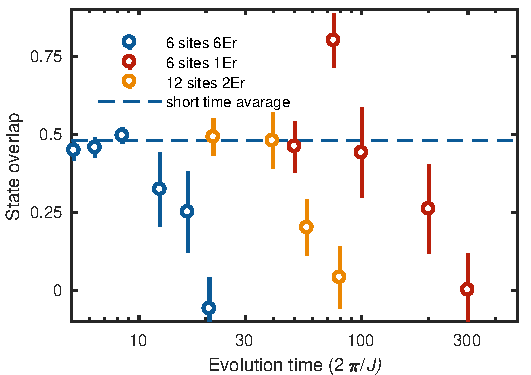
\includegraphics[scale=1]{figures/CBH_MBP_long_time.pdf}
	\caption{{\bf Long coherent dynamics in the system}. Quantum state overlap $Tr(\rho_1 \rho_2) $ for a system of $6$ atoms and various experimental parameters as a function of evolution time. Reducing the depth of the lattice along the chains increases the tunneling strength and decreases the differential disorder between two copies, resulting in increased the coherence time. The longest observed coherence of $\sim 100$ tunneling times shows an exquisite control over our experimental system.}
	\label{fig:CBH_MBP_long_time}
\end{figure*}

Since the quench populates a large fraction of the full Hilbert space of the system, above experiments show that we can precisely control the evolution of the system in $462$ dimensional Hilbert space over $\sim 100$ tunnelling times. We can also increase the effective Hilbert space size by increasing the number of available sites to the particles. To do that, we again prepare each copy with a string of $6$ atoms, but this time we confine them in the $12$ site long box, such that the atoms start at its centre. This increases the Hilbert space dimension of the system to $\sim 12 000$ eigenstates. We observe, that we can maintain the coherence between such a large number of states up to $\sim 40$ tunnelling times (see fig.~\ref{fig:CBH_MBP_long_time}). The decrease in the coherence time relative to the $6$ site long system might be due to the larger accumulation of differential tilts between two copies.  

\section{Coherence in the systems with single site control} 
Purity measurements provide a very sensitive probe for the optical potentials in our system, due to its stringent requirement on how identical the Hamiltonians of the copies should be in order to maintain the coherence. In order to test the performance of our DMD, we use the following procedure: Before starting the dynamics of the system, we use DMD to create an offset on one of the middle sites of both copies. If the applied potential is different between two chains, it will lead to the loss of coherence time in the system.

\begin{figure*}[t]
	\centering
	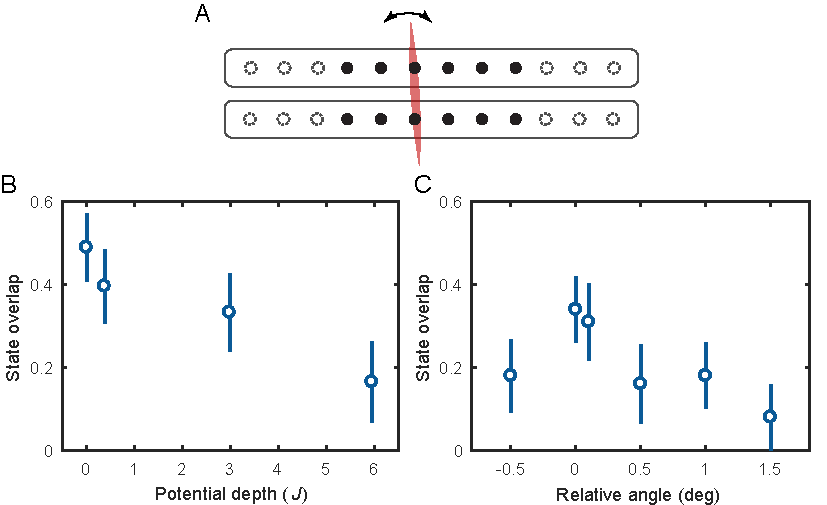
\includegraphics[scale=1]{figures/CBH_pattern_rotation_v2.pdf}
	\caption{{\bf Single site addressing with high precisions}. {\bf (A)} An additional single-site wide beam created by DMD is applied to system of $6$ atoms on $12$ sites, creating a potential offset on one site of each chin. Rotation of the pattern introduces a difference in the offsets experienced be each of the chains. {\bf (B)} Quantum state overlap $Tr(\rho_1 \rho_2)$ after $10$ tunneling times as a function of the applied potential depth, which is rotated be $0.5^{\circ}$. As the potential depth increases the state overlap decays due to the Hamiltonian difference between two chains. {\bf (C)} By rotating the pattern we can restore the overlap, once the potential is properly aligned to the system.}
	\label{fig:CBH_pattern_rotation}
\end{figure*}

We would like to determine the maximum height of the potential that can be applied before the copies start to decohere at $10$ tunnelling times. Note, that this timescale sets the relative precision of two potentials at $10^{-2}$ level. The potential we apply is a $2D$ Gaussian beam with a width of $1$ lattice site along the chain and $\sim 30$ sites in the transverse direction. Hence, we can intentionally make two copies slightly different by rotating the potential with respect to the copies. We start by applying a $0.5^{\circ}$ rotation and increase the depth of the potential until we see the purity decrease at the depth of $\sim 6\mathrm{J}$ (see fig.~\ref{fig:CBH_pattern_rotation}~B). Then we fix the depth of the potential to $6\mathrm{J}$ and measure the state overlap as a function of the relative angle to the lattice (see fig.~\ref{fig:CBH_pattern_rotation}~C). As we expect, the state overlap has a peak when the relative angle is zero, with FWHM $\sim 1^{\circ}$, which is consistent with numerical simulations for this parameter regime.

\section{Coherent evolution with a single copy}
In the previous sections, we have shown that we can prepare highly pure initial states and maintain their purity over two orders of time evolution. However, in order to achieve such outstanding performance we were restricted to work in a very shallow optical lattice, which can be an issue for certain types of experiments. The decoherence timescales observed with two copy method were consistent to be limited by the reduction in state overlap, due to the difference in the Hamiltonians between the copies. This means that our system might stay coherent over much longer timescales.

In any closed system, the decoherence of the state is always connected to some coupling of the system to the environment. Working with neutral atoms is a very good start since they only interact with the environment through collisions with photons or background atoms. As we have shown before, we can always overcome the latter by doing a post-selection on our state, and since we work with a far-detuned ($\sim 20 \mathrm{nm}$) optical potentials the probability of spontaneously scattering a photon is very low. We estimate the overall scattering rate in our system to be $\sim 0.012 \mathrm{Hz}$, which suggest that we should be able to maintain coherent evolution of $\sim 10$ particles over $\sim 1$ second.

\begin{figure*}[t]
	\centering
	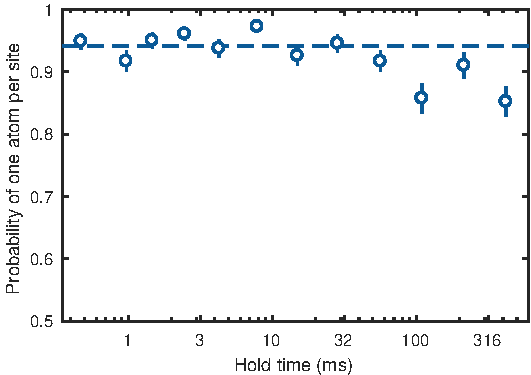
\includegraphics[scale=1]{figures/CBH_melt_and_back_p1.pdf}
	\caption{{\bf Probing coherence with a superfluid}. Starting with a unity filling Mott insulating chain of 8 atoms we adiabatically melt it into the superfluid state. After holding the superfluid for variable amount of time we adiabatically return the state back into the Mott regime, where we measure the probability of one particle on individual lattice sites averaged over the full chain of $8$ atoms. The dashed line shows the early time average from $1-10\mathrm{ms}$. Up to the longest measured time all points lay above a single excitation threshold of $0.75$.} 
	\label{fig:CBH_melt_and_back}
\end{figure*}

In order to probe the coherence in this case, instead of rapidly quenching the Hamiltonian parameters we adiabatically lower the lattice depth from deep in the Mott insulator phase into the superfluid phase, where atoms are allowed to tunnel. Since our Mott state is highly pure, it means that the system is occupying a single many-body state, in this case, it is a ground state of the system. Consequently, if we do adiabatic ramps into the superfluid and back we should still stay in the ground state of the system. Hence, any decoherence should result in the formation of excitations, which deep in the Mott phase result in the formation of doublone-hole pairs. In our experiment, we can detect those, by doing atom number resolved readout of the final sate.

In order to study the decoherence over time, we add a variable hold time in the superfluid regime. We observe that probability of one particle per lattice site stays constant over few hundred milliseconds (see fig.~\ref{fig:CBH_melt_and_back}), which is consistent with our overall scattering rate. This timescale suggests that we have coherent many-body dynamics over $\sim 500$ tunnelling times in a $2\mathrm{E_r}$ optical lattice.